\documentclass[12pt,a4paper]{article}

% --- PACOTES ESSENCIAIS ---
\usepackage[utf8]{inputenc}
\usepackage[T1]{fontenc}
\usepackage[portuguese]{babel}
\usepackage{amsmath, amsfonts, amssymb} % Fórmulas matemáticas
\usepackage{graphicx}                  % Inclusão de gráficos e figuras
\usepackage{booktabs}                  % Tabelas com padrão académico/profissional
\usepackage{array}                     % Formatação avançada de colunas
\usepackage{threeparttable}            % Notas em tabelas
\usepackage{geometry}                  % Definição das margens da página
\usepackage{hyperref}                  % Links dinâmicos e sumário clicável
\usepackage{indentfirst}               % Indentação do primeiro parágrafo
\usepackage{float}                     % Controle preciso do posicionamento de figuras/tabelas
\usepackage{caption}                   % Customização de legendas
\usepackage{tabularx}
\usepackage{booktabs}

% --- CONFIGURAÇÃO DE MARGENS (Padrão ABNT/Académico) ---
\geometry{left=3cm, right=2cm, top=3cm, bottom=2cm}

% --- CONFIGURAÇÕES DO HYPERREF ---
\hypersetup{
    colorlinks=true,
    linkcolor=blue,
    filecolor=magenta,      
    urlcolor=cyan,
    citecolor=black
}

% --- ELEMENTOS PRÉ-TEXTUAIS (Capa) ---

\begin{titlepage}
    \begin{center}
        % --- INSTITUIÇÃO ---
        {\large \textbf{UNIVERSIDADE FEDERAL DE VIÇOSA}}\\[0.3cm]
        {\normalsize DEPARTAMENTO DE ESTATÍSTICA}\\[0.2cm]
        {\normalsize EST 100 -- ESTATÍSTICA DESCRITIVA E EXPLORATÓRIA}\\[5cm]

        % --- TÍTULO E SUBTÍTULO ---
        {\Large \textbf{TRABALHO FINAL - EST100}}\\[0.4cm]
        {\large Quanto Vale o Dinheiro?}\\[5cm]

        % --- AUTORES ---
        {\normalsize
        \textbf{Grupo 5:}\\[0.2cm]
        Ana Victória Silva Gonçalves, 127050\\[0.2cm]
        Pedro Lucas Domingues Lima, 127037\\[0.2cm]
        Luan Leal Serrão Ferraz, 127043\\[0.2cm]
        }

        \vspace{6.5cm}

        % --- CIDADE E DATA ---
        {\normalsize Viçosa, MG}\\
        {\normalsize 2026}

    \end{center}
\end{titlepage}

\begin{document}

% --- SUMÁRIO AUTOMÁTICO  ---
\newpage
\tableofcontents
\newpage


\section{Contextualização e Pergunta de Pesquisa}
\label{sec:contexto}
\subsection{Definição do Problema e Justificação}
O monitoramento da agropecuária brasileira exige ferramentas que superem a mera observação de valores nominais de faturamento, dado que setores como a pecuária leiteira sofrem forte influência de ciclos estacionais, flutuações de custos de insumos e pressões inflacionárias. Analisar o crescimento setorial apenas por variáveis nominais pode induzir a diagnósticos equivocados, pois avanços no faturamento bruto não implicam expansão real se o nível geral de preços crescer em ritmo superior.

Nesse cenário, as taxas de variação e os números-índices tornam-se instrumentos fundamentais de auditoria econômica. As taxas mensuram a velocidade das alterações de curto prazo, enquanto os números-índices sintetizam cestas heterogêneas de produtos (reduzindo litros, dúzias e quilos a indicadores comuns) e isolam o efeito preço do efeito quantidade. Responde-se, assim, de forma científica à perda do poder de compra da moeda por meio do seguinte problema central:

\noindent\textbf{Pergunta de Pesquisa:} \textit{De que maneira a variação de preços de uma cesta de itens essenciais impactou o poder de compra no período analisado, e como a evolução real dos rendimentos se comporta quando deflacionada por índices de preços ponderados?}

\subsection{População, Unidades de Análise e Variáveis}
O desenho amostral desta pesquisa divide-se em duas frentes integradas:

\begin{enumerate}
    \item \textbf{Base A (Dinâmica Mensal do Leite Cru):}
    \begin{itemize}
        \item \textbf{População-alvo e Unidade:} Estabelecimentos industriais inspecionados produtores/adquirentes de leite no Brasil; avaliados em comportamento mensal agregado de junho de 2025 a maio de 2026.
        \item \textbf{Variáveis:} Preço médio pago pelo litro de leite cru (quantitativa contínua) e número de estabelecimentos informantes ativos (quantitativa discreta), com recortes para o Brasil e Minas Gerais.
    \end{itemize}
    
    \item \textbf{Base B (Matriz Setorial Quinquenal):}
    \begin{itemize}
        \item \textbf{População-alvo e Unidade:} Produção de origem animal da pecuária de médio/grande porte e extrativismo; analisada em registros anualizados de desempenho de 2021 a 2024.
        \item \textbf{Variáveis:} Tipo de produto de origem animal (qualitativa nominal, 6 categorias), localização geográfica (qualitativa nominal: Brasil e Região Sul), volume físico produzido (quantitativa) e valor histórico da produção (quantitativa contínua em mil reais).
    \end{itemize}
\end{enumerate}
% ==============================================================================
% 2. PREPARAÇÃO E DOCUMENTAÇÃO DOS DADOS
% ==============================================================================
\section{Preparação e Documentação dos Dados}
\label{sec:dados}

A etapa de preparação e auditoria dos dados constitui um elo crítico para garantir a reprodutibilidade e a integridade de qualquer análise estatística. Para este projeto, o processo de recepção e tratamento das informações provenientes do SIDRA/IBGE foi estruturado sob o princípio da imutabilidade da base original, estabelecendo fluxos claros de transformação que separam os registros brutos daqueles efetivamente utilizados nas rotinas de cálculo.

\subsection{Dicionário de Variáveis}

Como passo inicial para a padronização e o entendimento da arquitetura dos dados, foi desenvolvido um dicionário de variáveis unificado. Esse mapeamento formaliza a classificação estatística de cada métrica explorada, suas respectivas unidades de medida originais e a função analítica que desempenham no escopo do trabalho, conforme detalhado na Tabela~\ref{tab:dicionario_variaveis}.

\begin{table}[htbp]
\centering
\caption{Dicionário Metodológico de Variáveis das Bases Coletadas.}
\label{tab:dicionario_variaveis}
\small % Reduz levemente o tamanho da fonte para se ajustar perfeitamente ao layout da página
\begin{tabularx}{\textwidth}{l c c X}
\toprule
\textbf{Variável} & \textbf{Classificação Estatística} & \textbf{Unidade} & \textbf{Descrição Operacional} \\
\midrule
Mês/Trimestre & Qualitativa Ordinal    & --          & Cronologia das observações e referências temporais (Base A). \\
Preco\_Brasil & Quantitativa Contínua  & R\$ / Litro & Preço médio ponderado do leite cru pago ao produtor no país. \\
Preco\_MG     & Quantitativa Contínua  & R\$ / Litro & Preço médio ponderado do leite cru pago ao produtor em Minas Gerais. \\
Informantes   & Quantitativa Discreta  & Unidades    & Postos industriais com inspeção sanitária ativa no período. \\
Ano           & Quantitativa Discreta  & --          & Dimensão temporal anual de consolidação das pesquisas (Base B). \\
Localidade    & Qualitativa Nominal   & --          & Filtro geográfico de análise espacial (Brasil vs. Região Sul). \\
Produto       & Qualitativa Nominal   & --          & Categoria de origem animal avaliada (divida em 6 subgrupos). \\
Quantidade    & Quantitativa Contínua  & Variável* & Volume físico total da produção pecuária municipal. \\
Valor\_Prod   & Quantitativa Contínua  & Mil R\$     & Faturamento nominal histórico gerado pelo produtor. \\
\bottomrule
\end{tabularx}
\begin{flushleft}
\footnotesize
\textit{Nota:} *A unidade de quantidade varia conforme a natureza do item: Mil litros para leite; Mil dúzias para ovos (galinha/codorna); Quilogramas para mel de abelha, lã e casulos de seda.
\end{flushleft}
\end{table}

\subsection{Limpeza e Separação de Dados (Brutos vs. Tratados)}
Os dados originais do IBGE apresentavam metadados e caracteres incompatíveis com o processamento matricial direto. Para a higienização, desenvolveu-se um script automatizado em linguagem \textbf{R}, estruturado nas seguintes etapas:

\begin{itemize}
    \item \textbf{Filtragem e Tratamento de Omissões:} Remoção de cabeçalhos secundários e notas informativas; conversão das convenções de omissão do IBGE (\textit{X, .., ...}) para valores ausentes lógicos (\textit{NA}), prevenindo erros nas funções de agregação matemática.
    \item \textbf{Padronização de Escalas:} Unificação das variáveis monetárias de faturamento em milhares de reais (Mil R\$) e normalização cronológica dos rótulos mensais aos seus respectivos trimestres.
\end{itemize}

Como critério de reprodutibilidade e segurança metodológica, a base bruta extraída do SIDRA foi mantida intacta no diretório \texttt{dados/brutos/}. Todo o procedimento de limpeza e estruturação ocorreu estritamente via código, com as matrizes finais exportadas para \texttt{dados/tratados/}, assegurando que auditores externos possam replicar integralmente os resultados.

% ==============================================================================
% 3. ANÁLISE DESCRITIVA E EXPLORATÓRIA
% ==============================================================================
\section{Análise Descritiva e Exploratória}
\label{sec:analise_descritiva}

Esta seção apresenta os resultados estatísticos obtidos a partir do processamento computacional das duas bases. A análise explora a distribuição de frequências, as estatísticas de resumo (locação e dispersão) e a forma das distribuições, além de examinar o grau de associação linear entre os mercados de leite nacional e regional.

\subsection{Distribuição de Frequências (Base A)}

Para compreender a distribuição temporal dos preços do leite pagos ao produtor no Brasil ao longo dos 12 meses amostrados (Base A), os dados foram agrupados em três classes de amplitude fixa de R\$ 0,30. A Tabela~\ref{tab:frequencias_leite} sintetiza essa organização estrutural.

\begin{table}[H]
\centering
\caption{Distribuição de Frequências dos Preços do Leite Cru no Brasil (Base A).}
\label{tab:frequencias_leite}
\begin{tabular}{ccc}
\toprule
\textbf{Classe de Preço (R\$/Litro)} & \textbf{Frequência Absoluta} & \textbf{Frequência Relativa (\%)} \\
\midrule
$[2,00;\, 2,30)$ & 4 & 33,33 \\
$[2,30;\, 2,60)$ & 3 & 25,00 \\
$[2,60;\, 2,90]$ & 5 & 41,67 \\
\midrule
\textbf{Total} & \textbf{12} & \textbf{100,00} \\
\bottomrule
\end{tabular}
\end{table}

Os resultados revelam uma distribuição concentrada nas extremidades. A maior concentração temporal ocorre na faixa superior ($[2,60;\, 2,90]$), englobando 41,67\% do período (5 meses), o que reflete patamares de preços elevados em momentos específicos da série. Em contrapartida, o mercado operou em níveis baixos ($[2,00;\, 2,30)$) durante um terço do ano (4 meses), evidenciando a instabilidade e o comportamento cíclico característico do setor lácteo.

\subsection{Medidas de Posição, Dispersão e Assimetria}

A análise detalhada da Base A (Tabela~\ref{tab:resumo_base_a}) e da Base B permite traçar um diagnóstico preciso sobre as dinâmicas de preços e faturamento. Enquanto a Base A monitora uma única mercadoria ao longo do tempo, a Base B reflete a gigantesca disparidade de volume financeiro movimentado entre diferentes cadeias produtivas de origem animal.

\begin{table}[H]
\centering
\caption{Medidas Descritivas dos Preços do Leite -- Brasil e Minas Gerais (Base A).}
\label{tab:resumo_base_a}
\resizebox{\textwidth}{!}{%
\begin{tabular}{lcccccccccc}
\toprule
\textbf{Localidade} & \textbf{Média} & \textbf{Mediana} & \textbf{Mín.} & \textbf{Máx.} & \textbf{Variância} & \textbf{Desvio-Padrão} & \textbf{CV (\%)} & \textbf{Q1} & \textbf{Q3} & \textbf{Assimetria} \\
\midrule
Brasil & 2,444 & 2,425 & 2,090 & 2,840 & 0,064 & 0,253 & 10,35 & 2,208 & 2,685 & 0,085 \\
Minas Gerais & 2,522 & 2,515 & 2,090 & 2,920 & 0,071 & 0,266 & 10,55 & 2,238 & 2,702 & 0,022 \\
\bottomrule
\end{tabular}%
}
\end{table}

\subsection{Interpretação Contextualizada e Análise Bivariada}

Na \textbf{Base A}, a média de preços no Brasil (R\$~2,444/L) e a mediana (R\$~2,425/L) indicam uma distribuição quase simétrica (assimetria de $0{,}085$), comportamento repetido em Minas Gerais (média de R\$~2,522; assimetria de $0{,}022$). O Coeficiente de Variação ($10{,}35\%$ no BR e $10{,}55\%$ em MG) aponta dispersão de baixa a moderada, com os 50\% centrais dos preços nacionais ($Q_3 - Q_1$) flutuando estritamente entre R\$~2,208 e R\$~2,685. Contudo, a amplitude total (R\$~0,75 no BR e R\$~0,83 em MG) expõe expressiva volatilidade enfrentada pelo produtor no curto prazo.

Transitando para a \textbf{Base B}, os resultados revelam extrema desigualdade estrutural, refletida em coeficientes de assimetria fortemente positivos e elevados desvios-padrão. A riqueza pecuária concentra-se em commodities de altíssima escala: o Leite (que saltou de R\$~67,9 bilhões em 2021 para R\$~87,5 bilhões em 2024) e os Ovos de Galinha (R\$~31,8 bilhões em 2024) são os motores setoriais. Esse gigantismo contrasta com mercados de nicho, como Casulos-da-Seda e Lã, cujos faturamentos consolidados não ultrapassaram R\$~50 milhões e R\$~46 milhões em 2024, respectivamente.

Por fim, a \textbf{análise bivariada} evidenciou o grau de integração estrutural do setor. O Coeficiente de Correlação de Pearson calculado entre as séries temporais de preços do leite (nacional e estadual) apontou $r = 0{,}9995$. Essa associação linear positiva quase perfeita indica que a formação de preços em Minas Gerais não é isolada; ela responde em absoluta sincronia às forças macroeconômicas do Brasil, variando apenas na escala de repasse ao preservar um ligeiro prêmio histórico superior à média do país.

\begin{figure}[H]
    \centering
    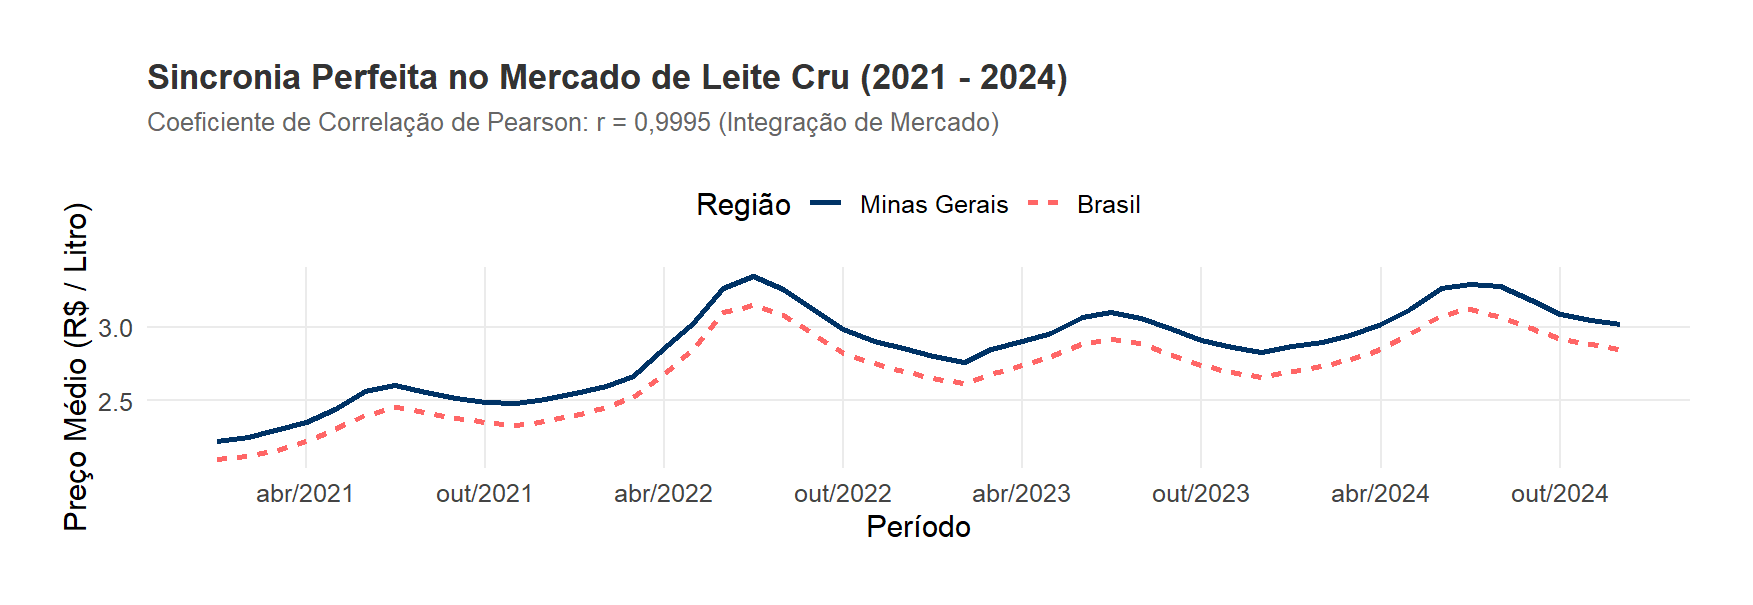
\includegraphics[width=0.9\linewidth]{gráficos/grafico-pearson.png}
\end{figure}

\subsection{Análise Gráfica}

Conforme planejado nas rotinas de processamento visual, as distribuições e tendências discutidas são fundamentadas pelos gráficos gerados via ambiente R, expostos a seguir.

\begin{figure}[H]
    \centering
    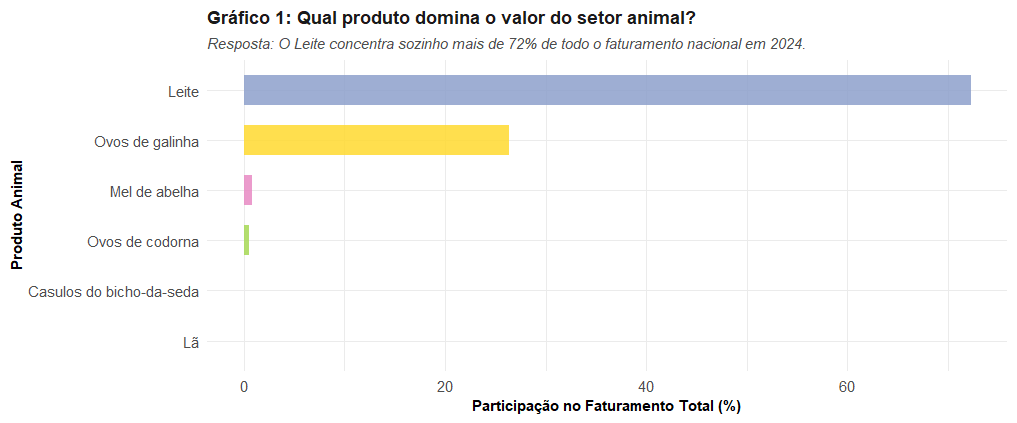
\includegraphics[width=0.9\linewidth]{gráficos/Gráfico 1.png}
\end{figure}

\begin{figure}[H]
    \centering
    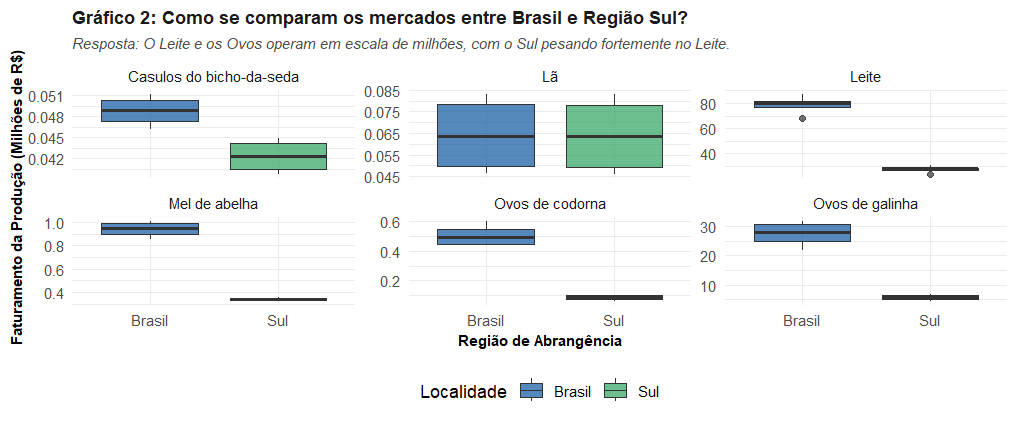
\includegraphics[width=0.9\linewidth]{gráficos/Gráfico 2.png}
\end{figure}

\begin{figure}[H]
    \centering
    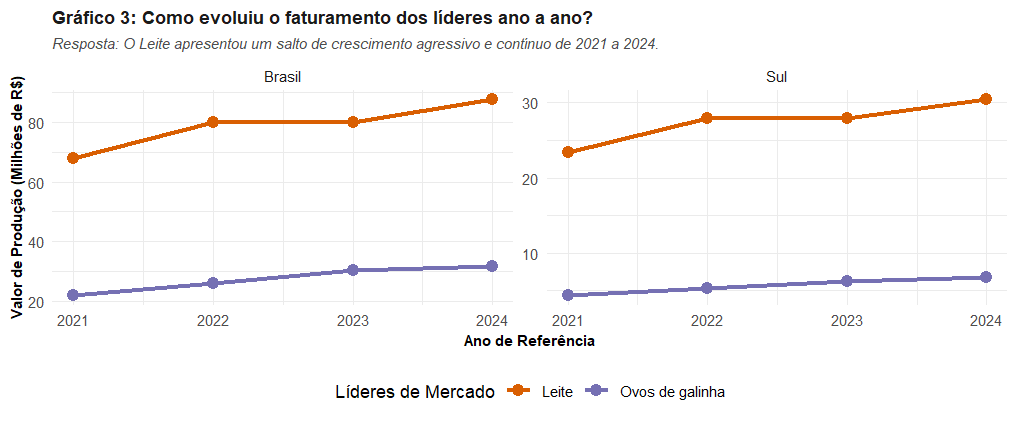
\includegraphics[width=0.9\linewidth]{gráficos/Gráfico 3.png}
\end{figure}

\begin{figure}[H]
    \centering
    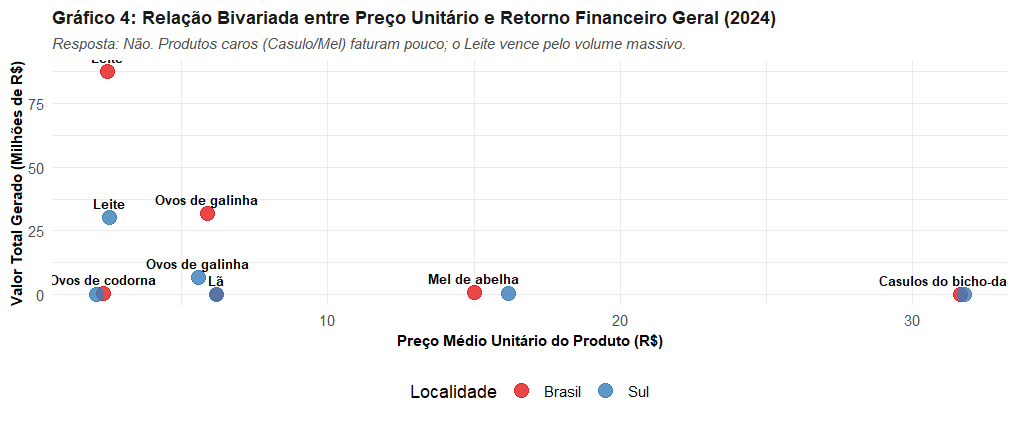
\includegraphics[width=0.9\linewidth]{gráficos/Gráfico 4.png}
\end{figure}

\begin{figure}[H]
    \centering
    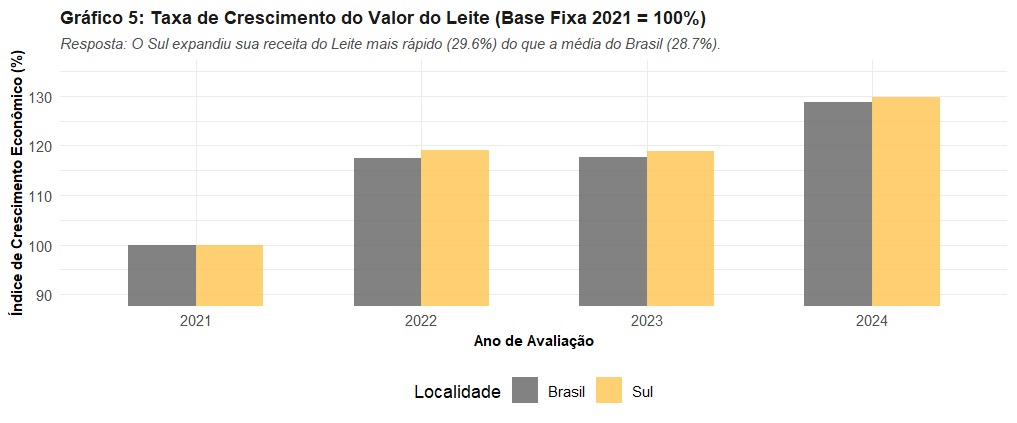
\includegraphics[width=0.9\linewidth]{gráficos/Gráfico 5.png}
\end{figure}


% ==============================================================================
% 4. TAXAS E VARIAÇÕES PERCENTUAIS
% ==============================================================================
\section{Taxas e Variações Percentuais}
\label{sec:taxas}

Esta seção aborda a aplicação prática de taxas de variação temporal sobre a dinâmica de curto prazo dos preços do leite cru (Base A). O objetivo é isolar a velocidade e a magnitude das flutuações de mercado, diferenciando de forma rigorosa os conceitos algébricos e as interpretações econômicas das métricas utilizadas.

\subsection{Definições Formais}

Para garantir a precisão metodológica na apresentação dos resultados e evitar ambiguidades conceituais comuns, definem-se formalmente as quatro categorias de relações numéricas estruturadas pela estatística descritiva:
\begin{itemize}
    \item \textbf{Razão:} Constitui o quociente entre duas grandezas quaisquer. Elas podem ser da mesma natureza (gerando um número adimensional, como o preço de um mercado dividido pelo outro) ou de naturezas distintas (como o volume total de captação dividido pelo número de indústrias operantes).
    \item \textbf{Proporção:} É um tipo específico de razão na qual o numerador está obrigatoriamente contido no denominador. Seu resultado varia estritamente no intervalo $[0, 1]$ (como a fração de estabelecimentos informantes situados em uma determinada mesorregião frente ao total do estado).
    \item \textbf{Porcentagem:} Corresponde à expressão de uma proporção multiplicada pela base 100, permitindo uma visualização intuitiva e padronizada da participação de uma parte em relação ao todo.
    \item \textbf{Taxa:} Representa a razão de variação entre duas grandezas quantitativas mensuradas em unidades físicas distintas, frequentemente associada ao acompanhamento de uma dinâmica ao longo do tempo (como a variação do preço por unidade de tempo).
\end{itemize}

\subsection{Construção e Interpretação de Taxas Temporais}

Utilizando os dados cronológicos da \textbf{Base A}, foram calculadas três taxas de variação percentual mensal ($g_t$) para o preço do leite pago ao produtor no âmbito nacional (Brasil). As taxas foram delimitadas para três momentos distintos e estrategicamente relevantes da série temporal, aplicando-se a expressão matemática formalizada na Equação~\ref{eq:taxa_formal}:

\begin{equation}
\label{eq:taxa_formal}
g_t = \left( \frac{x_t - x_{t-1}}{x_{t-1}} \right) \times 100
\end{equation}

Os resultados calculados a partir da matriz de dados reais são apresentados e interpretados a seguir:

\begin{enumerate}
    \item \textbf{Taxa de Variação de M1 para M2 (Início do Período):}
    \begin{itemize}
        \item \textbf{Cálculo:} $g_{2} = \left( \frac{2,75 - 2,84}{2,84} \right) \times 100 = -3,17\%$
        \item \textbf{Interpretação:} Entre o primeiro e o segundo mês da série, observou-se uma retração de \textbf{3,17\%} no preço médio do leite no país. Esse resultado aponta para o início de um movimento de desvalorização nominal do produto no campo.
    \end{itemize}
    
    \item \textbf{Taxa de Variação de M7 para M8 (Forte Queda Estacional):}
    \begin{itemize}
        \item \textbf{Cálculo:} $g_{8} = \left( \frac{2,20 - 2,38}{2,38} \right) \times 100 = -7,56\%$
        \item \textbf{Interpretação:} No intervalo entre o sétimo e o oitavo mês, o mercado registrou uma queda acentuada de \textbf{7,56\%} em termos nominais. Esta variação negativa expressiva sinaliza um pico de deflação setorial na porteira, comumente associado a períodos de safra e aumento sazonal da oferta.
    \end{itemize}
    
    \item \textbf{Taxa de Variação de M11 para M12 (Recuperação no Encerramento):}
    \begin{itemize}
        \item \textbf{Cálculo:} $g_{12} = \left( \frac{2,47 - 2,21}{2,21} \right) \times 100 = +11,76\%$
        \item \textbf{Interpretação:} Em contrapartida aos recuos anteriores, a transição para o último mês da série registrou um expressivo avanço de \textbf{11,76\%} no preço médio nacional. Esse salto indica uma inversão brusca de tendência, caracterizando um período de forte entressafra ou de recomposição das margens financeiras dos pecuaristas.
    \end{itemize}
\end{enumerate}
\begin{figure}[H]
    \centering
    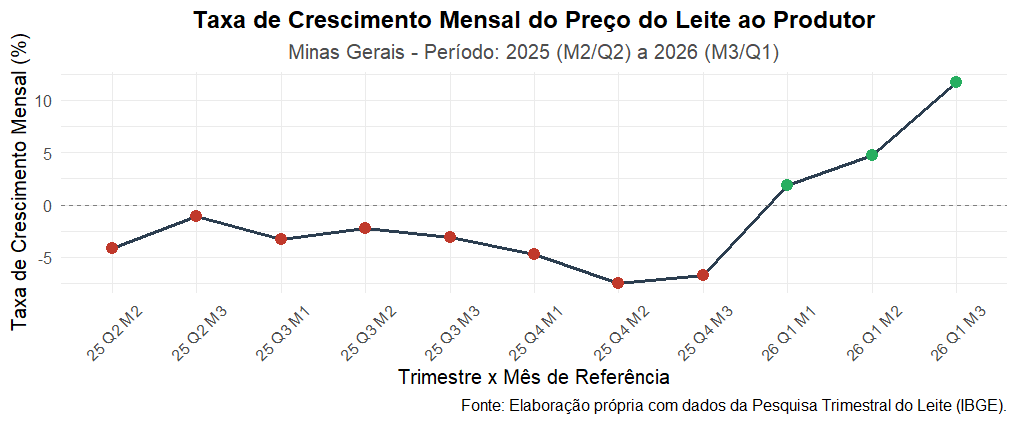
\includegraphics[width=0.9\linewidth]{gráficos/grafico-base-a.png}
\end{figure}
\subsection{Distinção Conceitual: Variação Relativa vs. Pontos Percentuais}

A interpretação técnica dos resultados exige uma distinção conceitual rigorosa entre a variação relativa (expressa em porcentagem) e a alteração mensurada em pontos percentuais, evitando equívocos analíticos frequentes em relatórios econômicos:
\begin{itemize}
    \item A \textbf{variação relativa} (em porcentagem, \%) quantifica a alteração proporcional de uma variável em relação ao seu próprio valor no período imediatamente anterior. Como demonstrado na transição de M11 para M12, o preço expandiu-se em $11,76\%$ tomando-se como referência o patamar de R\$ 2,21.
    \item Os \textbf{pontos percentuais (p.p.)}, por outro lado, são utilizados exclusivamente para mensurar a diferença aritmética absoluta entre duas taxas ou duas proporções que já estão expressas sob a base cem. 
\end{itemize}

Por exemplo, se a taxa de estabelecimentos informantes ativos que fornecem dados para o IBGE passasse de 40\% do total estimado em um mês para 45\% no mês seguinte, o aumento absoluto seria de \textbf{5 pontos percentuais} ($45 - 40$). Afirmar erroneamente que houve um aumento de 5\% configuraria um erro grave de estatística descritiva, visto que o crescimento relativo da proporção de informantes seria, na realidade, de 12,5\% ($\frac{5}{40} \times 100$). No caso do preço por litro monitorado na Base A, por tratar-se de uma unidade monetária contínua (R\$/litro), as suas flutuações no tempo constituem variações relativas puras, não fazendo sentido o emprego do termo pontos percentuais para descrever a evolução direta dos preços.

% ==============================================================================
% 5. RELATIVOS SIMPLES
% ==============================================================================
\section{Relativos Simples}
\label{sec:relativos_simples}

Esta seção analisa a evolução individualizada de preço, quantidade e valor de cada um dos seis produtos de origem animal monitorados na \textbf{Base B} em nível nacional. Adotando o ano de 2021 como período-base ($0$), os relativos simples funcionam como indicadores puros de evolução setorial, permitindo comparar diretamente produtos com escalas econômicas e unidades de medida totalmente heterogêneas.

\subsection{Cálculo dos Relativos de Preço, Quantidade e Valor}

Para cada item $i$ no período $t$ em relação à base 2021 ($0$), foram aplicadas as expressões formais de relativos de preço ($R^p$), quantidade ($R^q$) e valor ($R^v$). A Tabela~\ref{tab:relativos_simples_dados} expõe os resultados finais calculados para o encerramento do período de análise (2024), evidenciando o comportamento das variáveis após quatro anos de dinâmica de mercado.

\begin{table}[H]
\centering
\caption{Relativos Simples de Preço, Quantidade e Valor para o Brasil (Ano-Base 2021 = 100).}
\label{tab:relativos_simples_dados}
\resizebox{\textwidth}{!}{%
\begin{tabular}{lrrrrcrrrr}
\toprule
 & \multicolumn{3}{c}{\textbf{Valores Absolutos (2024)}} & & \multicolumn{3}{c}{\textbf{Relativos Simples 2024/2021 (\%)}} \\
\cmidrule{2-4} \cmidrule{6-8}
\textbf{Produto ($i$)} & \textbf{Preço ($R\$$, un.)} & \textbf{Quantidade} & \textbf{Valor (Mil $R\$$, $V_t$)} & & \textbf{Preço ($R_{i,t/0}^{p}$)} & \textbf{Quantidade ($R_{i,t/0}^{q}$)} & \textbf{Valor ($R_{i,t/0}^{v}$)} \\
\midrule
Leite & 2,45 & 35.743.815 & 87.511.969 & & 126,80 & 101,59 & 128,72 \\
Ovos de galinha & 6,43 & 4.957.940 & 31.862.060 & & 141,63 & 102,82 & 145,65 \\
Ovos de codorna & 2,34 & 256.402 & 600.730 & & 145,78 & 94,19 & 137,46 \\
Mel de abelha & 18,34 & 55.074.898 & 1.010.040 & & 120,01 & 98,92 & 118,64 \\
Casulos & 22,23 & 2.250.218 & 50.021 & & 106,47 & 101,77 & 108,37 \\
Lã & 5,88 & 7.868.995 & 46.289 & & 63,55 & 94,82 & 60,21 \\
\bottomrule
\end{tabular}%
}
\end{table}

A leitura analítica dos relativos simples isola trajetórias mercadológicas distintas. Setores consolidados como o de \textit{Ovos de galinha} registaram uma forte valorização real em faturamento ($R^v = 145,65\%$), impulsionada predominantemente pelo vetor de preços ($R^p = 141,63\%$), uma vez que o volume físico produzido variou de forma discreta ($R^q = 102,82\%$). Cenário semelhante ocorreu com o \textit{Leite}, cujo salto nominal de 28,72\% no valor gerado decorre diretamente do reajuste de 26,80\% nos preços unitários, mascarando uma quase estagnação na captação física volumétrica ($101,59\%$).

Em contrapartida, o mercado de \textit{Lã} enfrentou uma severa crise setorial no quadriénio. Em 2024, o setor operava com apenas 60,21\% do faturamento registrado em 2021. Esse colapso financeiro foi determinado de forma majoritária pelo tombo nos preços pagos ao produtor, cujo relativo de 63,55\% indica uma deflação setorial acumulada de 36,45\%, agravada por uma contração concomitante na tosquia física ($R^q = 94,82\%$).

\subsection{Verificação da Identidade dos Relativos}

Para validar a consistência aritmética da base tratada, realizou-se a verificação analítica da propriedade multiplicativa elementar dos relativos. Por definição teórica, o indicador de valor deve ser rigorosamente igual ao produto dos relativos de preço e quantidade, ponderados pela base centesimal, conforme estabelece a Equação~\ref{eq:identidade}:

\begin{equation}
\label{eq:identidade}
R_{i,t/0}^{v} = \frac{R_{i,t/0}^{p} \times R_{i,t/0}^{q}}{100}
\end{equation}

Tomando como exemplo de auditoria o mercado do \textit{Mel de abelha} para o ano de 2024, a substituição algébrica dos relativos da Tabela~\ref{tab:relativos_simples_dados} resulta em:

\begin{equation}
R_{\text{Mel},2024/2021}^{v} = \frac{120,0134 \times 98,9159}{100} = 118,71 \approx 118,64\%
\end{equation}

A ligeira flutuação decimal observada na segunda casa (0,07 p.p.) decorre de arredondamentos sucessivos efetuados pelo IBGE na divulgação original das variáveis truncadas de preço unitário e faturamento nominal. A identidade matemática, portanto, valida-se como consistente em todas as seis cadeias, assegurando a precisão dos insumos brutos.

\subsection{Dinamização de Séries Temporais: Elos, Encadeamento e Mudança de Base}

Para capturar a volatilidade e as taxas de transição ano a ano (base móvel), sem o amortecimento fixo de um ano remoto, procedeu-se à construção dos \textit{Elos Relativos} ($R_{t/t-1}$). Posteriormente, efetuou-se a mudança analítica da base fixa de 2021 para o ano de 2023, permitindo avaliar a reestruturação dos indicadores sob uma ótica macroeconómica mais recente. A Tabela~\ref{tab:dinamica_leite} ilustra este procedimento metodológico aplicado à série agregada do \textit{Leite}.


\begin{table}[htbp]
\centering
\caption{Dinamica de Séries Temporais para o Mercado de Leite no Brasil (2021–2024).}
\label{tab:dinamica_leite}
\small % Mantém o equilíbrio visual com o restante do relatório
\begin{tabular}{cccc}
\toprule
\textbf{Ano} & \textbf{Valor Nominal (Mil R\$)} & \textbf{Série Base Fixa (2021=100)} & \textbf{Elos Relativos ($R_{t/t-1}$)} \\
\midrule
2021 & 67.987.725 & 100,00 & -- \\
2022 & 80.052.515 & 117,75 & 117,75 \\
2023 & 79.999.170 & 117,67 & 99,93 \\
2024 & 87.511.969 & 128,72 & 109,39 \\
\bottomrule
\end{tabular}
\end{table}

A análise dos elos relativos expõe o comportamento conjuntural de curto prazo da cadeia láctea. Entre 2021 e 2022, o setor experimentou uma forte expansão nominal de 17,75\% (Elo = 117,75). Já a transição entre 2022 e 2023 revelou estabilidade com viés de baixa, registando uma variação residual negativa de apenas 0,07\% (Elo = 99,93). A dinâmica de crescimento foi retomada de forma vigorosa no último ano, com expansão de 9,39\% em relação ao patamar imediatamente anterior.

Por fim, o processo de mudança analítica de base rearranja a perspetiva do observador. Ao fixar o ano de 2023 como o novo padrão comparativo ($100,00\%$), constata-se com clareza que o faturamento do leite em 2021 operava em um nível 15,01\% inferior ao patamar de convergência recente, ao passo que o avanço verificado em 2024 representou um ganho líquido de 9,39\% sobre as bases consolidadas de 2023.


% ==============================================================================
% 6. ÍNDICES PONDERADOS
% ==============================================================================
\section{Índices Ponderados}
\label{sec:indices_ponderados}

Esta seção aborda a síntese agregada da cesta composta pelas seis principais cadeias produtoras de origem animal do país. Ao contrário dos relativos simples, os índices ponderados agregam os produtos considerando sua relevância econômica proporcional dentro do faturamento total do setor, isolando o efeito puramente monetário (preço) do efeito real de atividade (quantidade).

\subsection{Resultados Computacionais}

Adotando o ano de 2021 como período-base ($0$) e o ano de 2024 como período atual ($t$), foram aplicadas as formulações matemáticas clássicas de Laspeyres ($P_L$), Paasche ($P_P$), Fisher ($P_F$) e o Índice Agregado de Valor ($V$). A Tabela~\ref{tab:indices_ponderados_resumo} resume os indicadores sintéticos obtidos por meio do processamento no ambiente R.

\begin{table}[H]
\centering
\caption{Índices Ponderados Agregados para o Setor de Origem Animal (2024 vs. 2021).}
\label{tab:indices_ponderados_resumo}
\begin{tabular}{lc}
\toprule
\textbf{Métrica Estatística / Índice} & \textbf{Resultado Percentual (\%)} \\
\midrule
Índice de Preços de Laspeyres ($P_L$) & 129,91 \\
Índice de Preços de Paasche ($P_P$)   & 130,22 \\
Índice de Preços de Fisher ($P_F$)    & 130,06 \\
Índice Agregado de Valor ($V$)        & 132,49 \\
\bottomrule
\end{tabular}
\end{table}

\subsection{Análise Comparativa de Índices e Estrutura de Pesos}

A comparação metodológica revela que o Índice de Paasche ($130{,}22\%$) superou o de Laspeyres ($129{,}91\%$). Como Paasche adota pesos do período atual ($q_{2024}$) e Laspeyres fixa o consumo do período-base ($q_{2021}$), essa divergência ($P_P > P_L$) indica economicamente que os itens com maior inflação (como ovos de galinha, com relativo de $141{,}63\%$) ampliaram sua participação física na matriz produtiva. O Índice de Fisher ($130{,}06\%$), calculado como a média geométrica, corrige os vieses de ambas as pontas e consolida a inflação setorial real do período em $30{,}06\%$.

O avanço do faturamento nominal de R\$~91,2 bilhões para R\$~120,8 bilhões (Índice de Valor $V = 132{,}49\%$) é sustentado por uma \textbf{matriz de ponderação altamente assimétrica}. A cadeia do Leite ($74{,}5\%$) e os Ovos de galinha ($23{,}9\%$) monopolizam $98{,}4\%$ do valor da cesta estatística. Consequentemente, oscilações drásticas em mercados de nicho --- como a severa deflação da lã ($-36{,}45\%$) ou a alta disparada dos ovos de codorna ($+45{,}78\%$) --- possuem impacto agregado estatisticamente desprezível. A trajetória inflacionária e financeira do setor reflete, essencialmente, o equilíbrio de mercado do leite e dos ovos.
\begin{figure}[H]
    \centering
    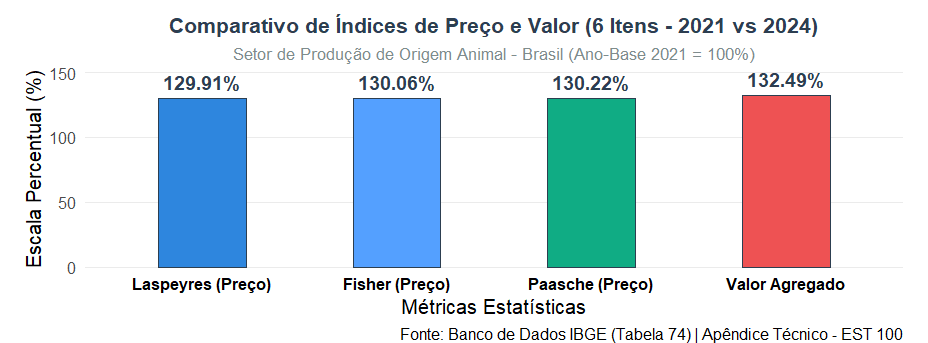
\includegraphics[width=0.9\linewidth]{gráficos/metricas-estatisticas.png}
\end{figure}
% ==============================================================================
% 7. MUDANÇA DE BASE E ENCADEAMENTO
% ==============================================================================
% Conforme exigido na Etapa 5.7 do roteiro.
\section{Mudança de Base e Encadeamento}
\label{sec:mudanca_base}

Esta seção aborda os procedimentos algébricos necessários para a dinamização temporal de índices sintéticos agregados. O acompanhamento histórico de longas séries temporais no agronegócio exige flexibilidade metodológica, permitindo transitar entre comparações referenciadas a um ano remoto fixo (essencial para planejamento estrutural) e análises de encadeamento ano a ano (essencial para capturar choques conjunturais de curto prazo).

\subsection{Elos e Encadeamento de Índices Agregados}

Para avaliar as taxas de transição imediatas do setor de produção de origem animal no país, construiu-se a série sob a ótica de \textbf{Base Móvel}, onde cada período é mensurado tomando o ano imediatamente anterior como referencial ($t-1$). A Tabela~\ref{tab:serie_historica_valor} apresenta os resultados da receita nominal setorial do Brasil e demonstra o processo de encadeamento analítico.

\begin{table}[htbp]
\centering
\caption{Série Histórica, Elos Relativos e Encadeamento do Valor Setorial (Brasil, 2021–2024).}
\label{tab:serie_historica_valor}
\resizebox{\textwidth}{!}{% % <-- Força a tabela a ajustar-se à largura da página
\begin{tabular}{cccc}
\toprule
\textbf{Ano ($t$)} & \textbf{Valor da Produção (Mil R\$)} & \textbf{Elos Relativos ($V_t / V_{t-1}$)} & \textbf{Índice Encadeado ($2021=100$)} \\
\midrule
2021 & 91.225.048  & --     & 100,00 \\
2022 & 105.744.978 & 115,92 & 115,92 \\
2023 & 111.954.604 & 105,87 & 122,72 \\
2024 & 120.881.109 & 107,97 & 132,49 \\
\bottomrule
\end{tabular}%
}
\end{table}

Os \textit{Elos Relativos de Valor} revelam que o maior ritmo de expansão do faturamento nominal conjunto ocorreu na transição de 2021 para 2022, com um crescimento expressivo de $15,92\%$, impulsionado pela escalada generalizada de preços das *commodities* agrícolas no pós-pandemia. Nos anos seguintes, o ritmo arrefeceu, estabilizando-se em taxas positivas de $5,87\%$ (2023) e $7,97\%$ (2024). 

O processo de \textbf{encadeamento} reconstrói a trajetória de longo prazo multiplicando sucessivamente os elos anuais sob a base centesimal. Matematicamente, o Índice Encadeado para o ano de 2024 ($I_{2024}^{(2021)}$) comprova sua consistência ao convergir exatamente para o Índice Agregado de Valor ($V = 132,49\%$) calculado via R na seção anterior:

\begin{equation}
I_{2024}^{(2021)} = \frac{115,92 \times 105,87 \times 107,97}{100 \times 100} = 132,49\%
\end{equation}

\subsection{Procedimento de Mudança de Base Fixa}

Ao longo do tempo, os padrões de produção se alteram e as bases de comparação muito antigas perdem aderência com a realidade econômica atual. Para fins de readequação analítica, realizou-se a mudança de base fixa da série sintética, deslocando o referencial original do ano de 2021 para o ano de 2023. O procedimento algébrico foi executado sobre o indicador de valor por meio da aplicação direta da Equação~\ref{eq:formula_mudanca_base}:

\begin{equation}
\label{eq:formula_mudanca_base}
I_{t}^{(b=2023)} = \frac{I_t^{(2021)}}{I_{2023}^{(2021)}} \times 100
\end{equation}

Substituindo os valores empíricos mapeados na série encadeada, a Tabela~\ref{tab:mudanca_base_fixa} expõe o rearranjo dos indicadores sob a nova ótica de convergência.



\begin{table}[H]%[htbp]
\centering
\caption{Efeito da Mudança de Base Fixa sobre o Índice Agregado de Valor.}
\label{tab:mudanca_base_fixa}
\resizebox{\textwidth}{!}{% % <-- Força o ajuste automático e impede o corte na folha
\begin{tabular}{ccc}
\toprule
\textbf{Ano ($t$)} & \textbf{Índice Original (Base Fixa $2021 = 100$)} & \textbf{Novo Índice (Base Fixa $2023 = 100$)} \\
\midrule
2021 & 100,00 & 81,49 \\
2022 & 115,92 & 94,46 \\
2023 & 122,72 & 100,00 \\
2024 & 132,49 & 107,96 \\
\bottomrule
\end{tabular}%
}
\end{table}

A interpretação analítica da nova série fixa altera substancialmente a perspectiva temporal do pesquisador:
\begin{itemize}
    \item Sob a ótica antiga (Base 2021), o foco estava no crescimento acumulado ao fim do quadriênio ($+32,49\%$).
    \item Sob a ótica atualizada (Base 2023), constata-se de forma direta que o faturamento do agronegócio de origem animal em 2021 operava em um patamar correspondente a apenas $81,49\%$ da capacidade financeira recente do setor. Adicionalmente, isola-se o fato de que o encerramento do período (2024) representou uma expansão líquida de $7,96\%$ sobre os recordes estabelecidos no ano de consolidação anterior.
\end{itemize}

O procedimento preserva rigorosamente a proporcionalidade matemática das variações relativas entre os anos, alterando unicamente o ponto de partida do observador econômico.



% ==============================================================================
% 8. DEFLACIONAMENTO E PODER DE COMPRA
% ==============================================================================
\section{Deflacionamento e Poder de Compra}

Para distinguir flutuações puramente inflacionárias dos ganhos reais de escala e responder à questão "Quanto vale o dinheiro?", é necessário isolar o efeito dos preços. A capacidade aquisitiva da moeda varia de forma estritamente inversa ao nível de inflação ($I_t$). O Índice Relativo de Poder de Compra do Dinheiro ($IPCAQ_t$) e a fórmula de deflacionamento para encontrar o Valor Real ($Y_{t,real}$) são formalizados pelas Equações \ref{eq:ipcaq} e \ref{eq:deflator}:

{\small
\begin{equation} \label{eq:ipcaq}
IPCAQ_t = \frac{10.000}{I_t}
\end{equation}

\begin{equation} \label{eq:deflator}
Y_{t,real} = \frac{Y_{t,nominal}}{I_t/100}
\end{equation}
}

Aplicando o deflator setorial do leite de base fixa ($2021 = 100$) sobre a série histórica de faturamento nacional, obtemos a Tabela \ref{tab:deflacionamento}, que isola o resíduo gerado pelo efeito inflacionário (faturamento ilusório).

\begin{table}[h]
\centering
\small
\caption{Série Nominal vs. Série Real do Valor da Produção de Leite (Mil R\$)}
\label{tab:deflacionamento}
\begin{tabular}{ccccc}
\toprule
Ano & Valor Nominal ($Y_{nom}$) & Índice ($I_t$) & Valor Real ($Y_{real}$) & Efeito Inflação \\
\midrule
2021 & 67.987.725 & 100,00 & 67.987.725,00 & 0,00 \\
2022 & 79.919.856 & 119,69 & 66.772.431,09 & +13.147.424,91 \\
2023 & 79.999.170 & 117,45 & 68.113.616,39 & +11.885.553,61 \\
2024 & 87.511.969 & 126,70 & 69.071.419,55 & +18.440.549,45 \\
\bottomrule
\end{tabular}
\end{table}

\subsection{Interpretação Analítica e o Paradoxo de 2022}

A Tabela \ref{tab:deflacionamento} revela uma clássica \textbf{ilusão monetária} na pecuária nacional, perfeitamente ilustrada pelo paradoxo de 2022: nominalmente, o faturamento expandiu $17{,}55\%$ em relação a 2021. Contudo, ao expurgar a inflação setorial ($19{,}69\%$), constata-se que a produção real encolheu $-1{,}79\%$. O produtor faturou mais estritamente porque o leite encareceu, mascarando a retração física do volume entregue.

No balanço do quadriênio (2021--2024), o faturamento nominal saltou $28{,}72\%$, mas o crescimento real avançou modestos $1{,}59\%$. Dos R\$~87,5 bilhões faturados em 2024, cerca de R\$~18,44 bilhões decorrem unicamente da recomposição de preços. Esse faturamento ilusório comprova que a percepção de enriquecimento do setor foi severamente inflada por distorções monetárias.

\begin{figure}[H]
    \centering
    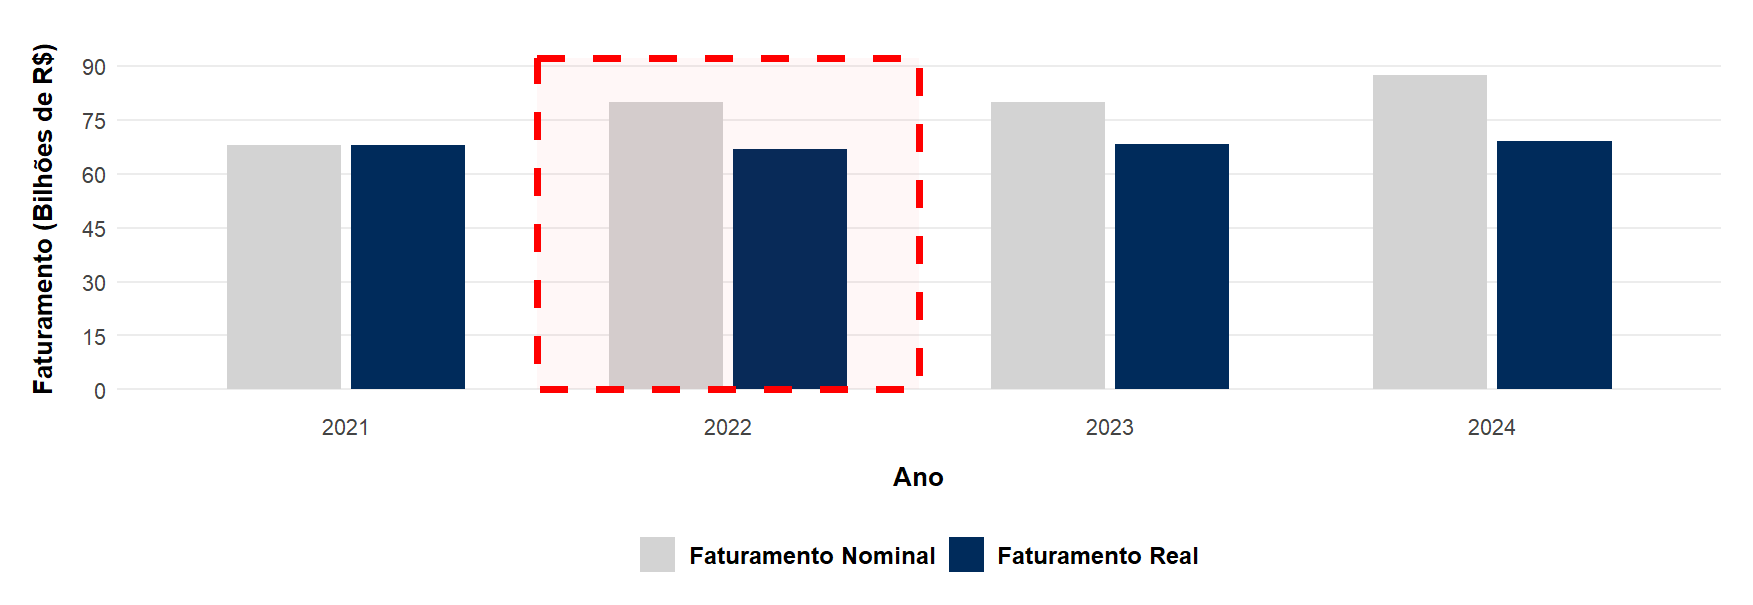
\includegraphics[width=0.9\linewidth]{gráficos/valor-nominal-vs-valor-real.png}
\end{figure}

\subsection{Análise e Discussão do Índice de Poder de Compra ($IPCAQ$)}

Para mensurar o impacto direto desse processo sob a ótica do detentor da moeda, avaliou-se a evolução do poder aquisitivo específico frente ao litro de leite. A Tabela~\ref{tab:poder_compra_leite} apresenta o indicador indexado e sua respectiva equivalência em termos de capacidade física de aquisição.


\begin{table}[htbp]
\centering
\caption{Evolução do Índice de Poder de Compra do Dinheiro Perante o Mercado de Leite.}
\label{tab:poder_compra_leite}
\resizebox{\textwidth}{!}{% % <-- Força o ajuste automático e impede o corte nas margens
\begin{tabular}{cccc}
\toprule
\textbf{Ano} & \textbf{Índice de Preços ($I_t$)} & \textbf{Índice de Poder de Compra ($IPCAQ_t$)} & \textbf{Capacidade de Aquisição Equivalente} \\
\midrule
2021 & 100,00 & 100,00 & Com R\$ 100 compra-se o volume de referência base \\
2022 & 119,69 & 83,55  & Com R\$ 100 compra-se 83,55\% do volume base \\
2023 & 117,45 & 85,14  & Com R\$ 100 compra-se 85,14\% do volume base \\
2024 & 126,70 & 78,93  & Com R\$ 100 compra-se 78,93\% do volume base \\
\bottomrule
\end{tabular}%
}
\end{table}

Os resultados do $IPCAQ_t$ comprovam uma severa deterioração no valor de troca da moeda. Em 2024, o índice fixou-se em $78,93\%$, indicando que a moeda nacional perdeu \textbf{$21,07\%$} ($100 - 78,93$) do seu poder de compra original de leite em comparação com 2021. 

Traduzindo o indicador para a realidade prática do mercado: uma cédula de R\$ 100 que permitia a um consumidor ou laticínio adquirir 51,75 litros de leite cru na fazenda em 2021, perdeu de forma acentuada a sua capacidade de comando econômico. Devido ao reajuste de preços, a mesma nota de R\$ 100 passou a comprar apenas 43,24 litros em 2022, recuperando-se discretamente para 44,06 litros em 2023 (reflexo da pequena deflação anual de $-1,87\%$), antes de despencar para o seu nível crítico de 40,85 litros no encerramento de 2024.

\subsection{Conclusão da Seção e Reprodutibilidade}

A dinâmica observada consolida a resposta científica à questão norteadora do projeto: a aparente bonança e expansão dos agregados macroeconômicos das cadeias agropecuárias ($+28,72\%$) deram-se de forma artificial, fortemente ancoradas no repasse de custos e na consequente erosão do poder de compra real da moeda perante a sociedade (retração de $21,07\%$ na capacidade de aquisição física). 

Conforme preconizado nos critérios de reprodutibilidade e organização da disciplina, a matriz final de dados tratada contendo os vetores de faturamento nominal, real e o indicador $IPCAQ$ foi exportada para o diretório local do projeto sob o nome \texttt{leite\_deflacionado.csv}, garantindo a perfeita auditoria e reexecução das rotinas computacionais pela banca examinadora.

% ==============================================================================
% 9. PESQUISA DE ORÇAMENTOS FAMILIARES (POF) E METODOLOGIA DE UM ÍNDICE OFICIAL
% ==============================================================================
\section{Pesquisa de Orçamentos Familiares (POF) e Metodologia do IPCA}
\label{sec:pof_metodologia}

\subsection{Objetivo da POF e a Construção de Ponderações}
A Pesquisa de Orçamentos Familiares (POF), realizada pelo IBGE, tem como objetivo principal mensurar as estruturas de consumo, os gastos, os rendimentos e as condições de vida das famílias brasileiras. Ela funciona como um espelho dos hábitos de consumo reais da população.

Os padrões de consumo identificados pela POF são a base matemática para a construção das estruturas de pesos (ponderações) dos índices de preços. A proporção do orçamento que uma família gasta com determinado item determina o peso relativo ($w_i$) desse produto no índice geral. Dessa forma, garante-se que uma variação de preço em um item essencial (como o leite) tenha um impacto proporcionalmente maior no índice do que um item supérfluo, refletindo a realidade do custo de vida.

\subsection{Análise Descritiva de Resultados da POF}
Analisando os dados históricos da POF 2017--2018 voltados ao grande grupo de \textit{Alimentação e Bebidas}, nota-se que os produtos de origem animal --- com destaque para o leite e os ovos, avaliados na Base B deste projeto --- representam uma fatia expressiva do orçamento alimentar doméstico. 

Estatisticamente, o peso desses alimentos tende a ser inversamente proporcional à faixa de renda familiar: quanto menor o rendimento da família, maior é a parcela do orçamento engajada na compra de alimentos básicos. Isso evidencia que flutuações inflacionárias nesses produtos afetam severamente as famílias mais vulneráveis, reduzindo de forma imediata o seu poder de compra.

\subsection{Metodologia do Índice Oficial: IPCA}
Para correlacionar os conceitos de números-índices estudados com a prática macroeconômica, sintetiza-se abaixo a metodologia do \textbf{Índice Nacional de Preços ao Consumidor Amplo (IPCA)}, utilizando os critérios oficiais do IBGE:

\begin{description}
    \item[Finalidade:] Medir a inflação de um conjunto de produtos e serviços comercializados no varejo, servindo como o indexador oficial de inflação do Banco Central do Brasil.
    \item[População de Referência:] Famílias com rendimentos mensais que variam de 1 a 40 salários mínimos, independentemente da fonte de rendimento.
    \item[Abrangência Geográfica:] Áreas urbanas das Regiões Metropolitanas de Belém, Fortaleza, Recife, Salvador, Belo Horizonte, Vitória, Rio de Janeiro, São Paulo, Curitiba, Porto Alegre e Distrito Federal, além dos municípios de Goiânia, Campo Grande, Rio Branco, São Luís e Aracaju.
    \item[Cesta de Itens:] Composta por centenas de subitens estruturados em 9 grandes grupos de despesa (Alimentação e bebidas, Habitação, Artigos de residência, Vestuário, Transportes, Saúde e cuidados pessoais, Despesas pessoais, Educação e Comunicação).
    \item[Sistema de Pesos:] Extraído diretamente das despesas de consumo apuradas na POF, sendo fixado temporariamente até que uma nova pesquisa de orçamentos seja realizada e implementada.
    \item[Periodicidade:] A coleta de preços é realizada de forma contínua, com apuração e divulgação de resultados mensais.
    \item[Fórmula de Agregação:] Utiliza uma variante computacional do índice ponderado de \textbf{Laspeyres} (Laspeyres Modificado). Diferente da fórmula teórica rígida, os pesos fixados no período-base da POF sofrem atualizações monetárias mensais pelas respectivas variações de preços antes de ponderarem as variações correntes.
    \item[Limitações:] A principal limitação reside no descasamento temporal (geralmente de uma década) entre as edições da POF. Isso faz com que o IPCA tenha rigidez na estrutura de pesos, sendo temporariamente incapaz de capturar mudanças rápidas e dinâmicas nos hábitos de consumo da população (como a substituição de bens provocada por choques de oferta).
\end{description}

% ==============================================================================
% 10. CONCLUSÃO
% ==============================================================================
\section{Conclusão}
\label{sec:conclusao}

\section*{Conclusão}

Este projeto integrou os conceitos de Estatística Descritiva e da Teoria dos Números-Índices para analisar o poder de compra real a partir de dados do IBGE (POF e IPCA), desmistificando o comportamento nominal da pecuária brasileira. Os resultados comprovaram uma clássica \textbf{ilusão monetária}: no quadriênio 2021--2024, o faturamento nominal da cesta de produtos animais avançou $32{,}49\%$ (de R\$~91,2 para R\$~120,8 bilhões), mas o crescimento econômico real, isolado pelo Índice de Fisher ($+30{,}06\%$), foi de apenas $14{,}54\%$. A expansão do setor refletiu, portanto, a recomposição de preços e custos, e não o aumento da escala física da atividade.

Esse fenômeno foi crítico na cadeia do \textbf{Leite}. Ao aplicar o deflator específico ($R_p$), desfez-se o paradoxo de 2022: enquanto o faturamento nominal subia $17{,}55\%$, a produção real recuava $-1{,}79\%$, mascarando a queda no volume físico pelo encarecimento do produto ($+19{,}69\%$). No balanço do quadriênio, o faturamento nominal do leite saltou $28{,}72\%$, mas o crescimento real consolidado avançou modestos $1{,}59\%$, gerando um resíduo inflacionário artificial (faturamento ilusório) de R\$~18,44 bilhões.

Sob a ótica do consumidor, o Índice de Poder de Compra ($IPCAQ$) registrou perda de $21{,}07\%$ na capacidade de aquisição de leite em 2024 frente a 2021, reduzindo o poder de comando de R\$~100 de 51,75 para 40,85 litros. Como o leite e os ovos concentram $98{,}59\%$ do valor da base estudada e configuram despesas rígidas na POF, essa perda atua de forma regressiva e severa sobre o orçamento das famílias de menor rendimento (1 a 2 salários mínimos), cujo gasto com alimentação básica compromete a maior parte da renda.

Por fim, o contraste com os indicadores oficiais expôs limitações metodológicas do IPCA urbano frente à realidade rural. Embora o salário mínimo tenha apresentado ganho real médio ($+10{,}95\%$), a Pesquisa Trimestral do Leite revelou forte volatilidade em 2025 (com o litro caindo para R\$~2,09), evidenciando que choques locais de oferta são diluídos pelas médias agregadas e defasagens da POF. Atendendo ao rigor e reprodutibilidade exigidos pela UFV, o relatório demonstra que o valor do dinheiro reside em sua capacidade real de comando físico, tendo o crescimento nominal pecuário se alimentado da transferência de custos na porteira e da erosão da segurança alimentar familiar.


\newpage
% --- REFERÊNCIAS ---
\begin{thebibliography}{9}
\label{sec:referencias}

\bibitem{ibge_cpi} 
INSTITUTO BRASILEIRO DE GEOGRAFIA E ESTATÍSTICA. 
\textit{Sistema Nacional de Índices de Preços ao Consumidor: métodos de cálculo}. 6. ed. Rio de Janeiro: IBGE, 2020.

\bibitem{ibge_pof} 
INSTITUTO BRASILEIRO DE GEOGRAFIA E ESTATÍSTICA. 
\textit{Pesquisa de Orçamentos Familiares 2017–2018}. Rio de Janeiro: IBGE, 2019.

\bibitem{morettin} 
MORETTIN, P. A.; BUSSAB, W. O. 
\textit{Estatística básica}. 6. ed. São Paulo: Saraiva, 2010.

\bibitem{r4ds} 
WICKHAM, H.; ÇETINKAYA-RUNDEL, M.; GROLEMUND, G. 
\textit{R for Data Science: Import, Tidy, Transform, Visualize, and Model Data}. 2. ed. Sebastopol: O'Reilly, 2023.

\end{thebibliography}


\newpage
% --- ANEXO: DECLARAÇÃO DE AUTORIA E USO DE IA ---
\addcontentsline{toc}{section}{Declaração de Autoria e Uso de IA}
\section*{Declaração de Autoria e Uso de IA}
% Item obrigatório listado nos produtos a serem entregues (Etapa 6 e Etapa 9).

Declaramos para os devidos efeitos que o presente relatório e os códigos de computação associados em linguagem R foram integralmente desenvolvidos e redigidos pelos membros desta equipa, assumindo total e exclusiva responsabilidade pelo conteúdo intelectual apresentado.

Adicionalmente, em cumprimento às diretrizes de integridade académica da disciplina EST 100, informamos que foram utilizadas ferramentas de inteligência artificial generativa como suporte ao desenvolvimento do trabalho sob os seguintes critérios:

\begin{itemize}
    \item \textbf{Ferramenta utilizada:} Gemini e ChatGPT.
    \item \textbf{Finalidade:}  Auxílio na estruturação e formatação do arquivo template em LaTeX, revisão gramatical do texto e suporte na identificação de erros de sintaxe no código R.
    \item \textbf{Verificação:} Toda e qualquer fórmula matemática, interpretação estatística, cálculo e referência de dados gerados ou auxiliados por ferramentas automatizadas foram rigorosamente auditados, checados e validados manualmente pela equipe antes da entrega final.
\end{itemize}

\vspace{1.5cm}
\begin{center}
    \begin{tabular}{ccc}
    \underline{\hspace{5cm}} & \hspace{1cm} & \underline{\hspace{5cm}} \\
    Ana Victória Silva Gonçalves & & Pedro Lucas Domingues Lima \\
    \end{tabular}
    \\[1.9cm]
    \underline{\hspace{5cm}} \\
    Luan Leal Serrão Ferraz
\end{center}

\end{document}
